% Author: Izaak Neutelings (March 2021)
% page 8 https://archive.org/details/StaticAndDynamicElectricity
% https://tex.stackexchange.com/questions/56353/extract-x-y-coordinate-of-an-arbitrary-point-on-curve-in-tikz
% https://tex.stackexchange.com/questions/412899/tikz-calculate-and-store-the-euclidian-distance-between-two-coordinates
\documentclass[border=3pt,tikz]{standalone}
\usepackage{physics}
\usepackage{bm}
\usetikzlibrary{3d}
\usepackage{tikz,pgfplots}
\usetikzlibrary{calc}
\usetikzlibrary{intersections}
\usetikzlibrary{decorations.markings}
\tikzset{>=latex} % for LaTeX arrow head
\pgfplotsset{compat=1.13}
\usepackage{xcolor}
\colorlet{Ecol}{orange!90!black}
\colorlet{EcolFL}{orange!80!black}
\tikzstyle{charge+}=[very thin,top color=red!50,bottom color=red!90!black,shading angle=20]
\tikzstyle{charge-}=[very thin,top color=blue!50,bottom color=blue!80,shading angle=20]
\tikzset{EFieldLine/.style={thick,EcolFL,decoration={markings,mark=at position #1 with {\arrow{latex}}},
                                 postaction={decorate}},
         EFieldLine/.default=0.5,
         EFielLineArrow/.style args = {#1}{EcolFL,decoration={markings,
          mark=at position 0.5 with {\arrow[rotate=#1]{latex}}},
          postaction={decorate}}
}


\makeatletter
  \newcommand{\xy}[3]{% % FIND X, Y
    \tikz@scan@one@point\pgfutil@firstofone#1\relax
    \edef#2{\the\pgf@x}%
    \edef#3{\the\pgf@y}%
  }
\makeatother
\newcommand{\EFielLineArrow}[2]{ % ELECTRIC FIELD LINE ARROW
  \pgfkeys{/pgf/fpu,/pgf/fpu/output format=fixed} % for calculation between -1*10^324 and +1*10^324
  \pgfmathsetmacro{\x}{#1/28.45pt}
  \pgfmathsetmacro{\y}{#2/28.45pt}
  \pgfmathsetmacro{\U}{\Q*((\y+\a)^2+(\x)^2)^(3/2)}
  \pgfmathsetmacro{\V}{\q*((\y-\a)^2+(\x)^2)^(3/2)}
  \pgfkeys{/pgf/fpu=false}
  \pgfmathparse{
    atan2(((\y+\a)*\V+(\y-\a)*\U),((\x)*\V+(\x)*\U))
  }
  \edef\angle{\pgfmathresult}
  \pgfmathsetmacro{\D}{int(1000*\q*(\y+\a)/sqrt((\y+\a)^2+\x*\x) + 1000*\Q*(\y-\a)/sqrt((\y-\a)^2+\x*\x))/1000}
  \draw[EFielLineArrow={\angle}] (\xpt,\ypt);
}
\newcommand{\EFieldLines}{ % ELECTRIC FIELD LINES
  \message{^^JField lines (\q,\Q) with contours range ^^J\range^^J}
    
  % FIELD LINES
  \draw[EcolFL,name path=Elines] plot[id=plot, raw gnuplot, smooth]
    function{
       f(x,y) = \q*(y+\a)/sqrt((y+\a)**2+x**2) + \Q*(y-\a)/sqrt((y-\a)**2+x**2);
       set xrange [-\xmax:\xmax];
       set yrange [-\ymax:\ymax];
       set view 0,0;
       set isosample 400,400;
       set cont base;
       set cntrparam levels discrete \range;
       unset surface;
       splot f(x,y)
    };
  
  % ELLIPSE INTERSECTIONS
  %\path[name path=ellipse1] (0,-\a) ellipse ({1.6*\R} and {0.85*\R});
  \path[name path=ellipse2] (0,+\a) ellipse ({1.6*\R} and {0.85*\R});
  %\path[name path=ellipse3] (  0,0) ellipse ({\a+\R} and 1.5*\R);
  \foreach \c in {2}{
    \message{Intersections \c...}
    \path[name intersections={of=Elines and ellipse\c,total=\t}]
      \pgfextra{\xdef\Nb{\t}};
    \message{ found \Nb ^^J}
    \foreach \i in {1,...,\Nb}{
      \message{  \i}
      \xy{(intersection-\i)}{\xpt}{\ypt}
      \EFielLineArrow{\xpt}{\ypt}
      \message{ (\D,\x,\y)^^J}
    }
  }
}
\newcommand{\EFieldLinesDashed}{ % ELECTRIC FIELD LINES
  \message{^^JField lines (\q,\Q) with contours range ^^J\range^^J}
  \draw[EcolFL,dashed] plot[id=plot, raw gnuplot, smooth]
    function{
       f(x,y) = \q*(y+\a)/sqrt((y+\a)**2+x**2) + \Q*(y-\a)/sqrt((y-\a)**2+x**2);
       set xrange [-\xmax:\xmax];
       set yrange [-\ymax:\ymax];
       set view 0,0;
       set isosample 400,400;
       set cont base;
       set cntrparam levels discrete \range;
       unset surface;
       splot f(x,y)
    };
}


\begin{document}


% CHARGE IMAGE - PLANE
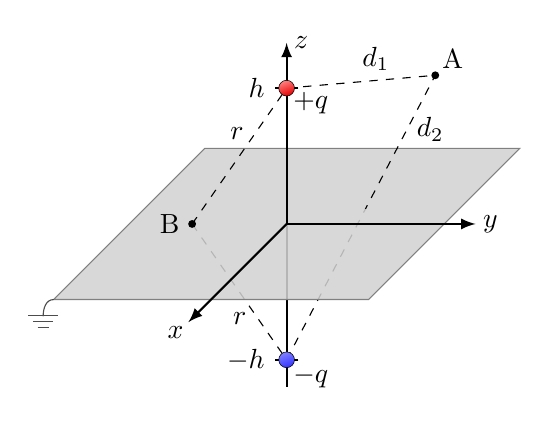
\begin{tikzpicture}[y={(0.5cm,0)},x={(-0.24cm,-0.24cm)},z={(0,0.5cm)}]
  \def\R{0.2}
  \def\L{4}
  \def\ymax{1.2*\L}
  \def\xmax{1.3*\L}
  \def\zmax{4.6}
  \def\pz{0.4} % z coordinate to determine intersection between line P'Q+ and plane
  \coordinate (Q+) at (0,0,0.75*\zmax);
  \coordinate (Q-) at (0,0,-0.75*\zmax);
  \coordinate (B) at (0,-0.6*\L,0);
  \coordinate (A) at (-0.3*\L,0.8*\L,0.8*\L);
  %\coordinate (P'') at (-0.2*\L,0.4*\L,0);
  %\coordinate (A) at ($(Q-)!1.5!(P'')$);
  
  % PLANE
  \draw[thick] (0,0,0) -- (0,0,-0.9*\zmax);
  \draw[dashed] (B) -- (Q-) node[pos=0.62,below left=-2] {$r$};
  \begin{scope}
    \clip (0,0,\pz) --++ (0,0,-\L) --++ (0,\L,0) --++ (0,0,\L) -- cycle;
    \draw[dashed] (Q-) -- (A);
  \end{scope}
  \fill[white,opacity=0.8]
    (\L,\L,0) -- (-\L,\L,0) -- (-\L,-\L,0) -- (\L,-\L,0) -- cycle;
  \fill[black!50,opacity=0.3]
    (\L,\L,0) -- (-\L,\L,0) -- (-\L,-\L,0) -- (\L,-\L,0) -- cycle;
  \draw[black!50]
    (\L,\L,0) -- (-\L,\L,0) -- (-\L,-\L,0) -- (\L,-\L,0) -- cycle;
  
  % GROUND
  \draw[black!70,line cap=round]
    (\L,-\L,0) to[out=180,in=90]++ (10:0.22*\L) coordinate (G);
  \foreach \i [evaluate={\y=(1-\i)*0.15; \w=0.5-\i*0.12;}] in {1,2,3}{
    \draw[black!70,canvas is yz plane at x=0]
      (G)++(-\w,\y) --++ (2*\w,0);
  }
  
  % AXES
  \draw[->,thick] (0,0,0) -- (\xmax,0,0) node[below left=-2] {$x$};
  \draw[->,thick] (0,0,0) -- (0,\ymax,0) node[right=-1] {$y$};
  \draw[->,thick] (0,0,0) -- (0,0,\zmax) node[right=-1] {$z$};
  \draw[thick] (Q+)++(0,0.3,0) --++ (0,-0.6,0) node[left] {$h$};
  \draw[thick] (Q-)++(0,0.3,0) --++ (0,-0.6,0) node[left] {$-h$};
  
  % POINT
  \draw[dashed] (B) -- (Q+) node[pos=0.59,above left=-2] {$r$};
  \draw[dashed] (Q+) -- (A) node[pos=0.6,above] {$d_1$};
  \begin{scope}
    \clip (0,0,\pz) --++ (0,0,\L) --++ (0,\L,0) --++ (0,0,-\L) -- cycle;
    \draw[dashed] (Q-) -- (A) node[pos=0.81,right=0] {$d_2$}; %{\contour{white}{$d_2$}};
  \end{scope}
  
  % CHARGE
  \draw[charge+,canvas is yz plane at x=0] (Q+) circle (\R) node[above=1,below right=-1] {$+q$};
  \draw[charge-,canvas is yz plane at x=0] (Q-) circle (\R) node[below right=-1] {$-q$};
  \fill[canvas is yz plane at x=0] (B) circle (0.1) node[left=1] {B};
  \fill[canvas is yz plane at x=0] (A) circle (0.1) node[above right=-1] {A};
  
\end{tikzpicture}


% CHARGE IMAGE - fieldlines
\begin{tikzpicture}
  \def\xmax{3}
  \def\ymax{2.5}
  \def\a{1.25}
  \def\q{-1}
  \def\Q{+1}
  \def\R{1.0}
  \def\N{5}
  %\def\range{-0.4,-1.0,-1.6}
  \def\range{-0.1,-0.4,-0.7,-1.0,-1.3,-1.6,-1.9}
  \begin{scope}
    \clip (-\xmax,0) rectangle (\xmax,\ymax);
    \EFieldLines
  \end{scope}
  \begin{scope} %[opacity=0.4]
    \clip (-\xmax,0) rectangle (\xmax,-\ymax);
    \EFieldLinesDashed
  \end{scope}
  \draw[charge+] (0,+\a) circle (0.2) node[black,scale=1.0] {$+$};
  \draw[charge-] (0,-\a) circle (0.2) node[black,scale=1.0] {$-$};
  \fill[white,opacity=0.6] (-\xmax,0) rectangle (\xmax,-\ymax);
  
  % PLATE & GROUND
  \fill[black!20] (-\xmax,-0.05*\R) rectangle (\xmax,0.05*\R);
  \draw[black!50]
    (-\xmax, 0.05*\R) --++ (2*\xmax,0)
    (-\xmax,-0.05*\R) --++ (2*\xmax,0);
  \draw[black!70,line cap=round]
    (-\xmax,-0.05*\R) to[out=180,in=90]++ (-140:0.12*\xmax) coordinate (G);
  \foreach \i [evaluate={\y=0.5*(1-\i)*0.15; \w=0.5*(0.5-\i*0.12);}] in {1,2,3}{
    \draw[black!70]
      (G)++(-\w,\y) --++ (2*\w,0);
  }
  \foreach \i [evaluate={\x=0.2+0.7*\xmax/\N*\i+0.55*\i^2/\N^2;}] in {0,...,\N}{
    \node[blue!80!black!80,scale=0.6] at (-\x,0) {$\bm-$};
    \node[blue!80!black!80,scale=0.6] at ( \x,0) {$\bm-$};
  }
\end{tikzpicture}


\end{document}
